\documentclass{article}
\usepackage[utf8]{inputenc}
\usepackage{minted}
\usepackage{graphicx}
\usepackage{hyperref}
\usepackage[dvipsnames]{xcolor}

\title{nanogateway lopy4 add node APB}
\author{cmonaton }
\date{August 2019}

\begin{document}

\maketitle





\section{Introduction}
But : Connecter un device à The Things Network par la méthode Activation By Personalisation. 
%Cette exemple est compatible avec une nanogateway lopy4.

Prérequis : savoir utiliser The Thing Network, cf tuto \textit{nanogateway\_lopy4\_lorawan}

Carte : pycom lopy 4 avec expansion board V3.0



\begin{figure}[H]
  \centering
  \begin{minipage}[b]{0.4\textwidth}
    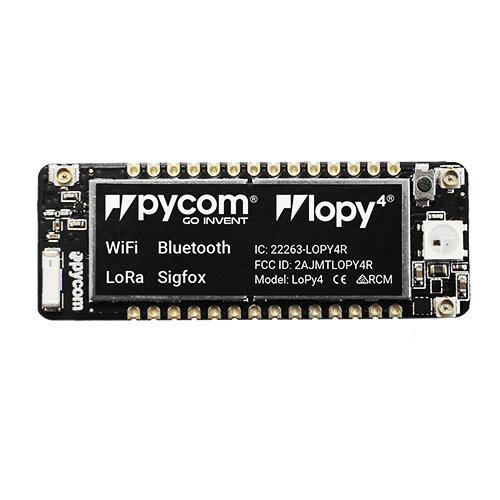
\includegraphics[keepaspectratio=true,scale=1.7]{pycom_lopy4.jpeg}
        \caption{pycom lopy 4}
  \end{minipage}
  \hfill
  \begin{minipage}[b]{0.4\textwidth}
   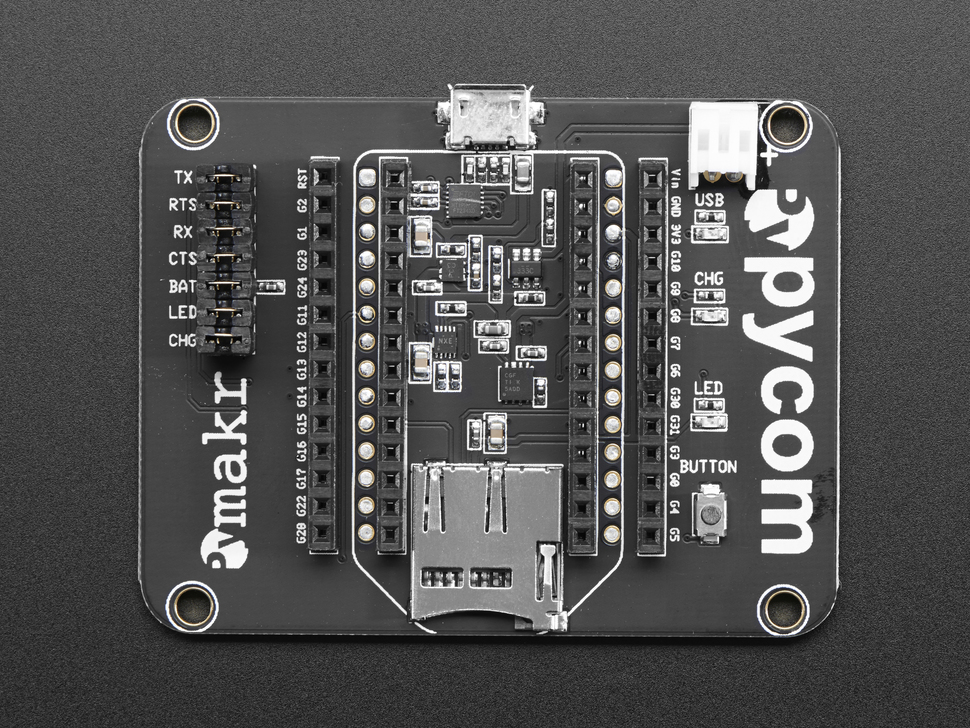
\includegraphics[keepaspectratio=true,scale=0.5]{pycom_expansion_board.jpeg}
    \caption{expansion board v3.0}
  \end{minipage}
\end{figure}

    \begin{figure}[H]
\begin{center}
\advance\leftskip-3cm
\advance\rightskip-3cm
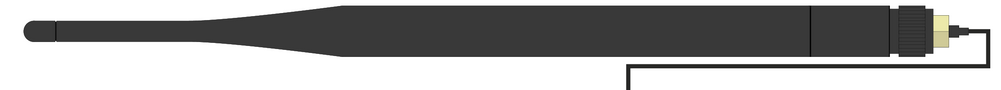
\includegraphics[keepaspectratio=true,scale=0.2]{lora_antenna.png}
\caption{antenne LoRa}
\label{visina8}
\end{center}\end{figure}



\section{Matériel}
\textcolor{red}{Branchez l'antenne LoRa avant d'alimenter la carte sinon la carte grille}





\section{Code pour Activation By Personalisation}



\textbf{Le code se trouve à : \url{https://github.com/CampusIoT/code-examples/tree/master/node_apb}}

Informations complémentaires : \url{https://docs.pycom.io/tutorials/lora/lorawan-nano-gateway/}\\

\subsection{Activation By Personalisation}
%Téléchargez le code suivant sur une carte lopy4+pymakr+antenne :

\begin{minted}{python}

""" ABP Node example compatible with the LoPy Nano Gateway """

from network import LoRa
import socket
import ubinascii
import struct
import time

# Initialise LoRa in LORAWAN mode.
lora = LoRa(mode=LoRa.LORAWAN,region=LoRa.EU868)

# create an ABP authentication params
dev_addr = struct.unpack(">l", ubinascii.unhexlify('2601147D'))[0] # these settings can 
#be found from TTN
nwk_swkey = ubinascii.unhexlify('3C74F4F40CAE2221303BC24284FCF3AF') # these settings can 
#be found from TTN
app_swkey = ubinascii.unhexlify('0FFA7072CC6FF69A102A0F39BEB0880F') # these settings can
#be found from TTN

# join a network using ABP (Activation By Personalisation)
lora.join(activation=LoRa.ABP, auth=(dev_addr, nwk_swkey, app_swkey))

# remove all the non-default channels
for i in range(3, 16):
    lora.remove_channel(i)

# set the 3 default channels to the same frequency
lora.add_channel(0, frequency=868100000, dr_min=0, dr_max=5)
lora.add_channel(1, frequency=868100000, dr_min=0, dr_max=5)
lora.add_channel(2, frequency=868100000, dr_min=0, dr_max=5)

# create a LoRa socket
s = socket.socket(socket.AF_LORA, socket.SOCK_RAW)

# set the LoRaWAN data rate
s.setsockopt(socket.SOL_LORA, socket.SO_DR, 5)

# make the socket non-blocking
s.setblocking(False)

""" Your own code can be written below! """

for i in range (200):
    s.send(b'PKT #' + bytes([i]))
    time.sleep(4)
    rx = s.recv(256)
    if rx:
        print(rx)
    time.sleep(6)



\end{minted}

\subsection{Créer une application sur The Thing Network}

\begin{itemize}


    \item Créez une application
    Depuis \textit{Console} sélectionner application, puis ajoutez une application :
    
    
    \begin{figure}[H]
\begin{center}
\advance\leftskip-3cm
\advance\rightskip-3cm
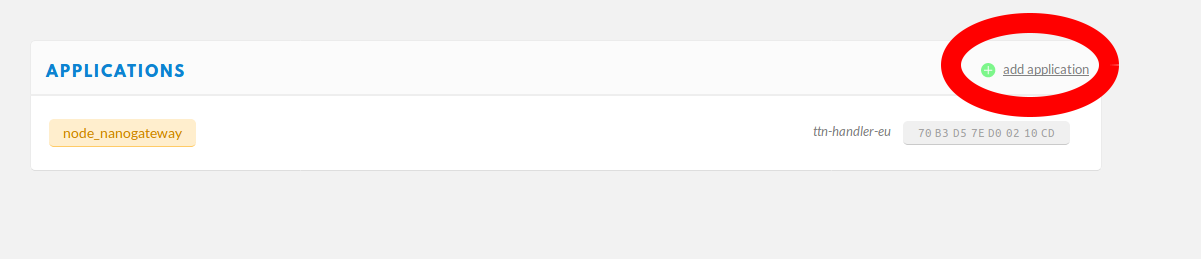
\includegraphics[keepaspectratio=true,scale=0.4]{add_appli.png}
\label{visina8}
\end{center}\end{figure}
    
    Donnez un nom pour l'application ID :
    
     \begin{figure}[H]
\begin{center}
\advance\leftskip-3cm
\advance\rightskip-3cm
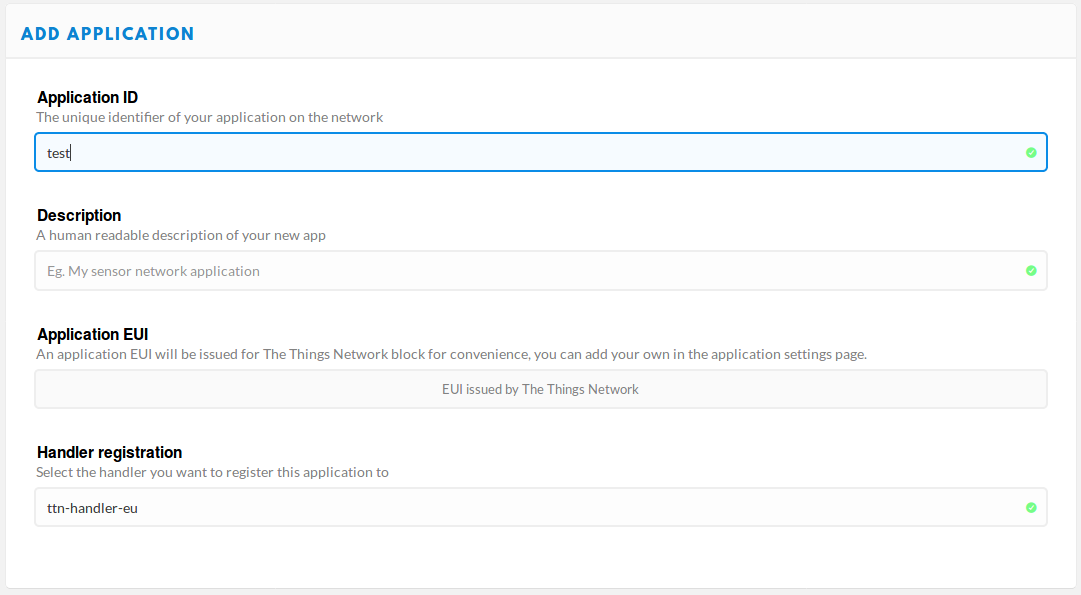
\includegraphics[keepaspectratio=true,scale=0.4]{appli_id.png}
\label{visina8}
\end{center}\end{figure}

\end{itemize}
    
    \subsection{Ajouter un device dans l'application}
    
        \begin{figure}[H]
\begin{center}
\advance\leftskip-3cm
\advance\rightskip-3cm
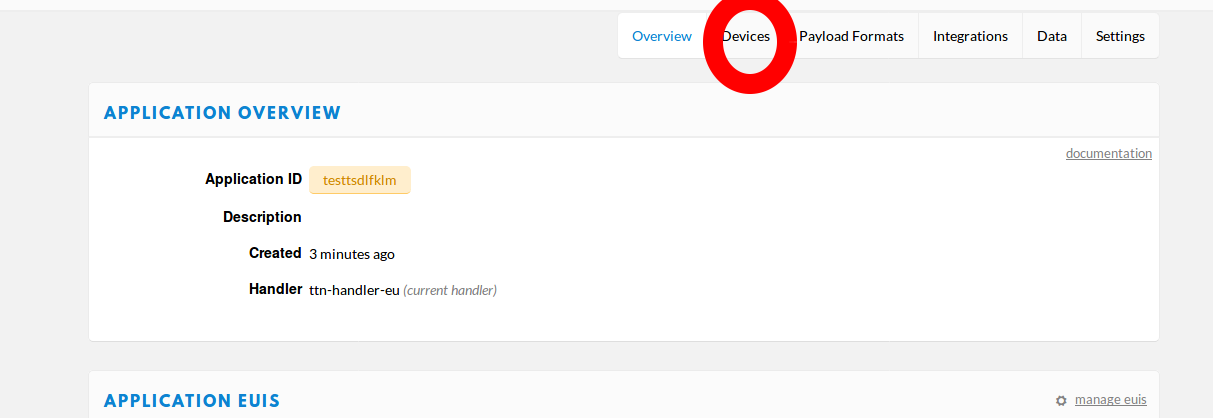
\includegraphics[keepaspectratio=true,scale=0.4]{add_device.png}
\label{visina8}
\end{center}\end{figure}

Puis \textit{register device} \\
Choisir un nom pour le device ID et 16 caractères hexadecimaux pour l'EUI.



 \begin{figure}[H]
\begin{center}
\advance\leftskip-3cm
\advance\rightskip-3cm
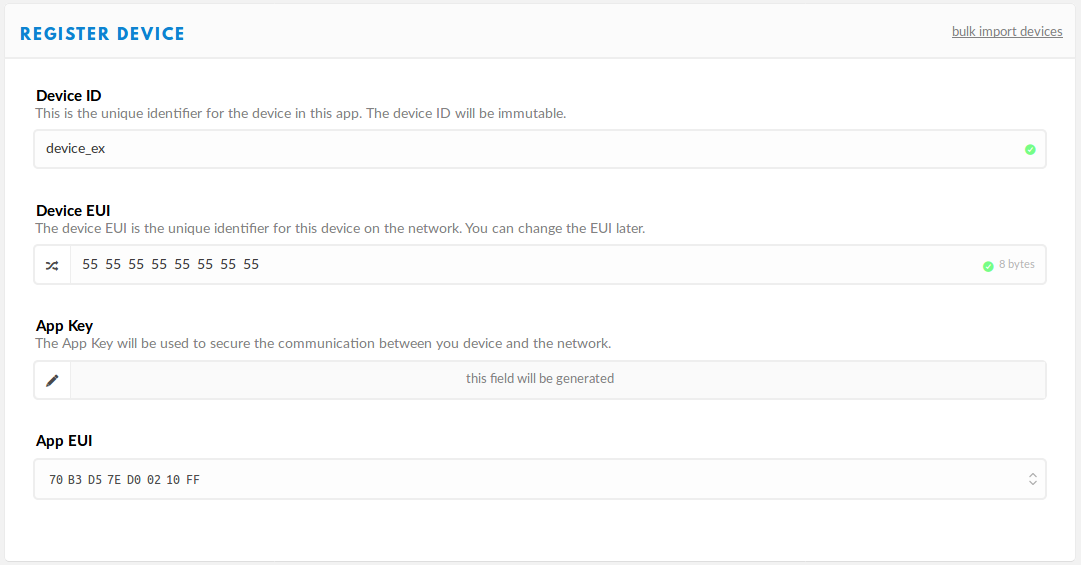
\includegraphics[keepaspectratio=true,scale=0.4]{device_ex_otaa.png}

\label{visina8}
\end{center}\end{figure}
 
 \subsubsection{Choisir APB comme méthode d'activation}
 Dans \textit{Device overview} allez dans \textit{settings}
 
  \begin{figure}[H]
\begin{center}
\advance\leftskip-3cm
\advance\rightskip-3cm
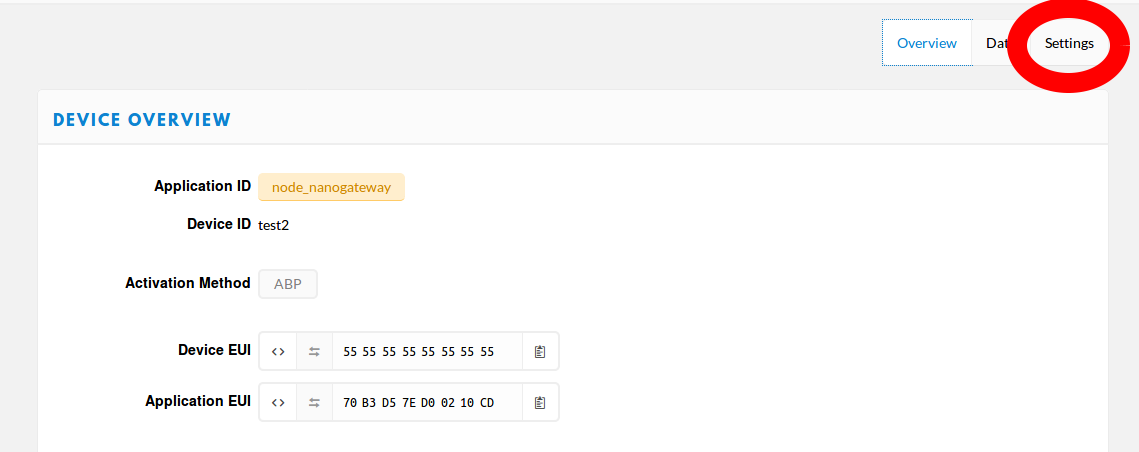
\includegraphics[keepaspectratio=true,scale=0.4]{settings_button_apb.png}

\label{visina8}
\end{center}\end{figure}
 
Puis entrez la network session key et l'application session key présents dans le code. 

\begin{figure}[H]
\begin{center}
\advance\leftskip-3cm
\advance\rightskip-3cm
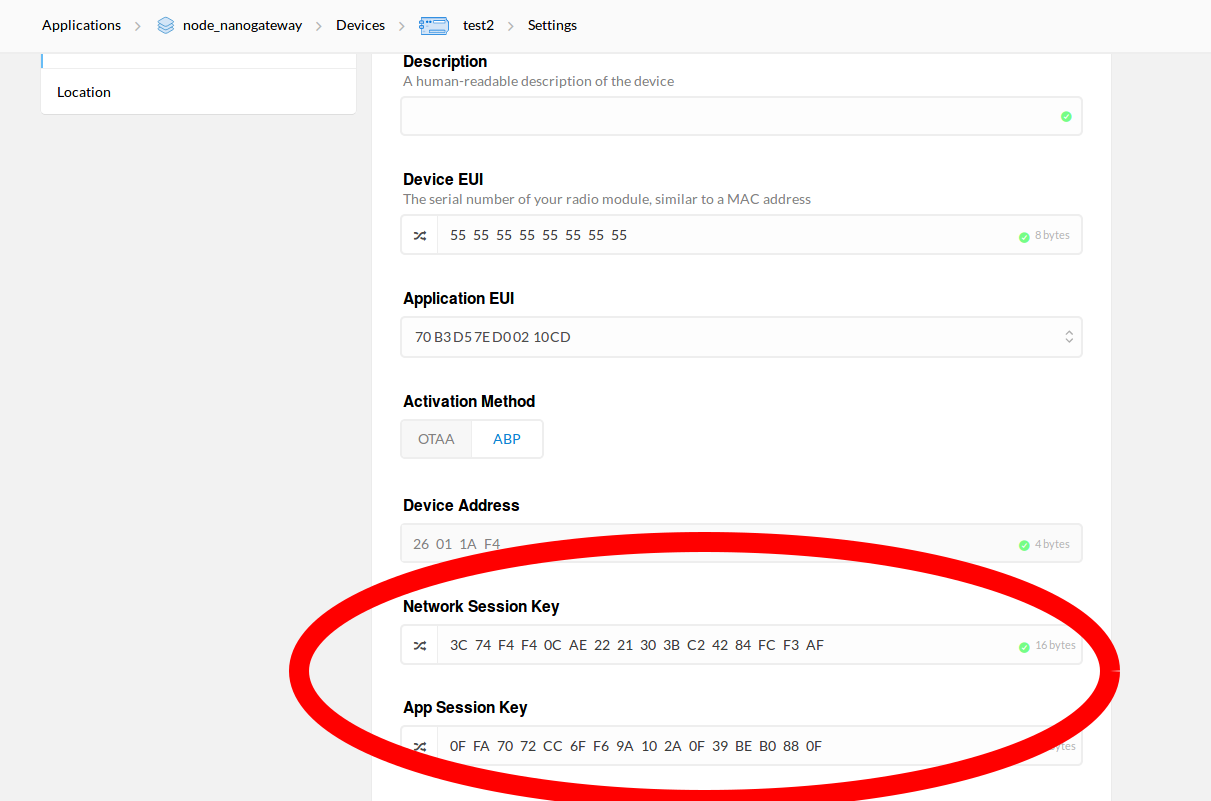
\includegraphics[keepaspectratio=true,scale=0.4]{settings_apb.png}
\label{visina8}
\end{center}\end{figure}

Bouton \textit{Save} puis revenez dans l'onglet \textit{Overview} et ajouter le device address dans le code.

\begin{figure}[H]
\begin{center}
\advance\leftskip-3cm
\advance\rightskip-3cm
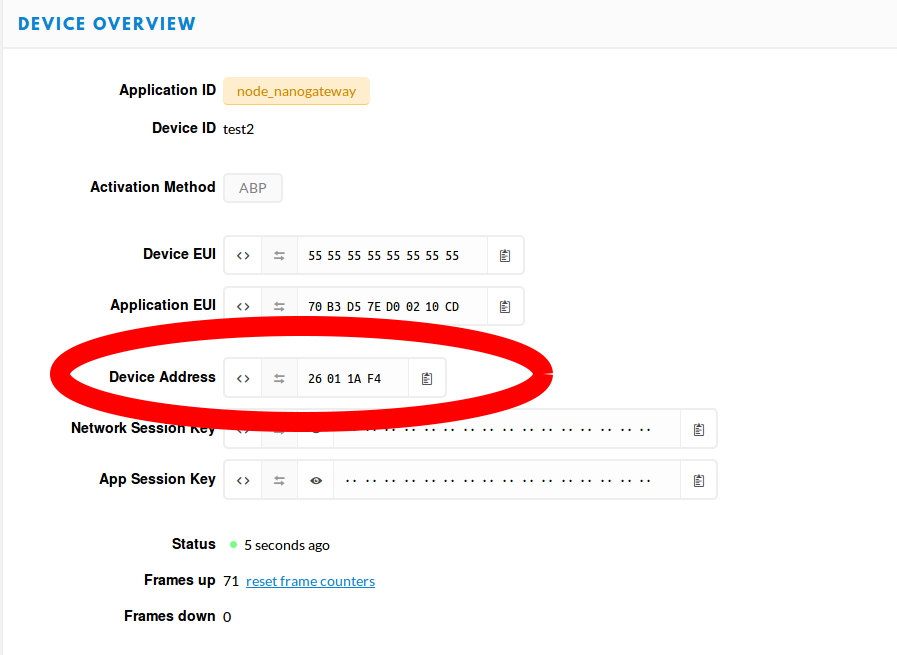
\includegraphics[keepaspectratio=true,scale=0.4]{overview_deviceaddressapb.png}
\label{visina8}
\end{center}\end{figure}

\textbf{Ajoutez Device address, network Session Key er App Session Key dans main.py}\\
Télécharger le code sur la carte.

    
    \subsection{Lire la payload envoyée par le device}
    
    \begin{itemize}
    \item Une fois le device connecté :

  \begin{figure}[H]
\begin{center}
\advance\leftskip-3cm
\advance\rightskip-3cm
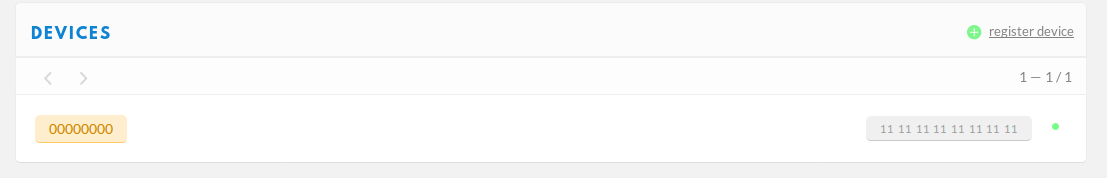
\includegraphics[keepaspectratio=true,scale=0.4]{device_connected.png}
\label{visina8}
\end{center}\end{figure}
  
  
  \item Dans l'onglet data :
  
  \begin{figure}[H]
\begin{center}
\advance\leftskip-3cm
\advance\rightskip-3cm
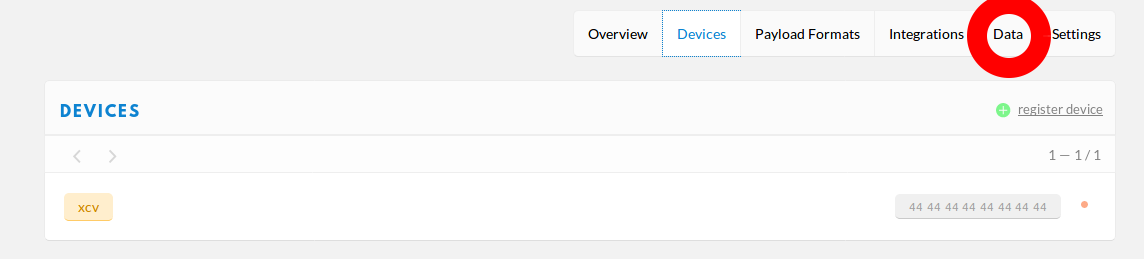
\includegraphics[keepaspectratio=true,scale=0.4]{data_tab.png}
\label{visina8}
\end{center}\end{figure}
  
  
  
  \begin{figure}[H]
\begin{center}
\advance\leftskip-3cm
\advance\rightskip-3cm
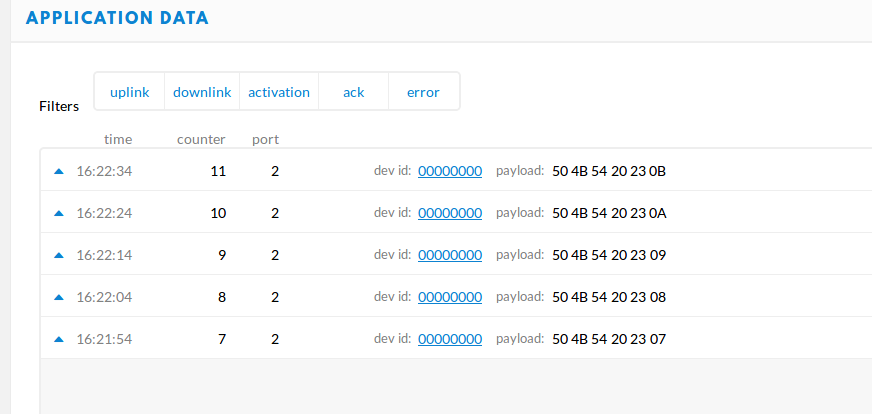
\includegraphics[keepaspectratio=true,scale=0.4]{payload.png}
\label{visina8}
\end{center}\end{figure}
  
  
\end{itemize}





\end{document}
